%%%%%%%%%%%%%%%%%%%%%%%%%%%%%%%%%%%%%%%%%%%%%%%%%%%%%%%%%%%%%%%%%%%%%%%%%%%%%%%
% STUDY NOTES
%%%%%%%%%%%%%%%%%%%%%%%%%%%%%%%%%%%%%%%%%%%%%%%%%%%%%%%%%%%%%%%%%%%%%%%%%%%%%%%

\documentclass[12pt]{paper}

\usepackage{amsmath}
\usepackage{amssymb}
\usepackage[
    backend=bibtex,
    style=numeric
]{biblatex}
\usepackage{booktabs}
\usepackage{chemformula}
\usepackage{fancyvrb}
\usepackage{hyperref}
\usepackage{geometry}
\usepackage{paralist}
\usepackage{pgfplots}
\usepackage{siunitx}
\usepackage{xfrac}

%%%%%%%%%%%%%%%%%%%%%%%%%%%%%%%%%%%%%%%%%%%%%%%%%%%%%%%%%%%%%%%%%%%%%%%%%%%%%%%
% CONFIGURATION
%%%%%%%%%%%%%%%%%%%%%%%%%%%%%%%%%%%%%%%%%%%%%%%%%%%%%%%%%%%%%%%%%%%%%%%%%%%%%%%

\geometry{margin=25mm}
\bibliography{references}

%%%%%%%%%%%%%%%%%%%%%%%%%%%%%%%%%%%%%%%%%%%%%%%%%%%%%%%%%%%%%%%%%%%%%%%%%%%%%%%
% COMMANDS
%%%%%%%%%%%%%%%%%%%%%%%%%%%%%%%%%%%%%%%%%%%%%%%%%%%%%%%%%%%%%%%%%%%%%%%%%%%%%%%

\newcommand{\newSection}[1]{\cleardoublepage\section{#1}}

%%%%%%%%%%%%%%%%%%%%%%%%%%%%%%%%%%%%%%%%%%%%%%%%%%%%%%%%%%%%%%%%%%%%%%%%%%%%%%%
% TITLE
%%%%%%%%%%%%%%%%%%%%%%%%%%%%%%%%%%%%%%%%%%%%%%%%%%%%%%%%%%%%%%%%%%%%%%%%%%%%%%%

\title{Study Notes}
\author{Walter Dal'Maz Silva}
\date{\today}

%%%%%%%%%%%%%%%%%%%%%%%%%%%%%%%%%%%%%%%%%%%%%%%%%%%%%%%%%%%%%%%%%%%%%%%%%%%%%%%
% DOCUMENT
%%%%%%%%%%%%%%%%%%%%%%%%%%%%%%%%%%%%%%%%%%%%%%%%%%%%%%%%%%%%%%%%%%%%%%%%%%%%%%%

\begin{document}
\maketitle%

\begin{abstract}
	This document has no specific or fixed structure. It is intended to be a single place to group study notes and short discussions about papers and books so that they can be reused later \emph{i.e.} to give a lecture or as reminder for a review for a paper. Please do not rely on this document as a perennial source or as a source of truth since there is no reviewer checking it to date.
\end{abstract}

\cleardoublepage\tableofcontents%

\newSection{Dynamical Systems}
\subsection{Fundamentals of linear systems}

A linear dynamical system of states $x\in\mathbb{R}^{n}$ is simply denoted in matrix form as $\dot{x}=\mathbf{A}x$, where $\mathbf{A}$ provides the dynamics. If an action $u\in\mathbb{R}^{m}$ is taken to control the system one might write it as $\dot{x}=\mathbf{A}x+\mathbf{B}u$. In this section we are mostly interested in the first formulation (without control) for which a general solution is $x(t)=\exp(\mathbf{A}t)x(0)$, where $\exp(\mathbf{A}t)$ is a matrix given by the Taylor series expansion:

\begin{equation}
\exp(\mathbf{A}t)=\mathbf{I}+\mathbf{A}t+\frac{\mathbf{A}^2t^2}{2!}+\frac{\mathbf{A}^3t^3}{3!}+\dots+\frac{\mathbf{A}^kt^k}{k!}
\end{equation}

Evaluation of this expression is non-trivial and good precision would require a large number of terms in the expansion. For linear systems the uncoupling of equations can be done through the eigenvalues and eigenvectors of $\mathbf{A}$ obtained by solving $\mathbf{A}\xi=\lambda\xi$. If we assembly a diagonal matrix $\mathbf{D}$ with eigenvalues and the column space of eigenvectors $\mathbf{T}$ as follows

\begin{equation}
\mathbf{D}=
\begin{bmatrix}
\lambda_{1} & & & \\
& \lambda_{2} & & \\
& & \ddots & \\
& & & \lambda_{n}
\end{bmatrix}
\qquad\text{and}\qquad
\mathbf{T}=
\begin{bmatrix}
\xi_{1} & \xi_{2} & \dots & \xi_{n}
\end{bmatrix}
\end{equation}

\noindent{}then we have $\mathbf{A}\mathbf{T}=\mathbf{T}\mathbf{D}$, which is easy to proof given the eigenvalue problem definition. We can use $\mathbf{T}$ to perform the transformations $x=\mathbf{T}z$ and $\dot{x}=\mathbf{T}\dot{z}$ from which the linear dynamical system can be written as $\mathbf{T}\dot{z}=\mathbf{A}\mathbf{T}z$ or reformulated as $\dot{z}=\mathbf{T}^{-1}\mathbf{A}\mathbf{T}z$. Since $\mathbf{D}=\mathbf{T}^{-1}\mathbf{A}$, the dynamics is fully uncoupled, \emph{i.e.} all equations become independent, and stated as $\dot{z}=\mathbf{D}z$. The solution of this system takes the same form as the coupled version, but now the evaluation of $\exp(\mathbf{D}t)$ which replaces $\exp(\mathbf{A}t)$ is a simple matrix as in

\begin{equation}
\exp(\mathbf{D}t)=
\begin{bmatrix}
	\exp(\lambda_{1}t) & & & \\
	& \exp(\lambda_{2}t) & & \\
	& & \ddots & \\
	& & & \exp(\lambda_{n}t)
\end{bmatrix}
\end{equation}

Reverting the solution back to physical space $x$ is quite simple. First we note that $\mathbf{A}=\mathbf{T}\mathbf{D}\mathbf{T}^{-1}$ what can be used to show that $\mathbf{A}^{k}=\mathbf{T}\mathbf{D}^{k}\mathbf{T}^{-1}$. This property can be used to demonstrate that $\exp(\mathbf{A}t)=\mathbf{T}\exp(\mathbf{D}t)\mathbf{T}^{-1}$. Thus, the problem solution can be rewritten as $x(t)=\mathbf{T}\exp(\mathbf{D}t)\mathbf{T}^{-1}x(0)$. By the definition of $z$ we have that $z(0)=\mathbf{T}^{-1}x(0)$, then $x(t)=\mathbf{T}\exp(\mathbf{D}t)z(0)$, but $z(t)=\exp(\mathbf{D}t)z(0)$ from which one finds the solution $x(t)=\mathbf{T}z(t)$.

\subsection{Stability of linear systems}

The main take from previous section is that the key features of a linear system dynamics is encoded in matrix $\mathbf{D}$, while eigenvectors in $\mathbf{T}$ are responsible by \emph{mixing modes} to produce the response in physical space. In fact, it is the exponential behavior $\exp(\lambda_{n}t)$ of eigenvalues $\lambda_{n}$ placed over the diagonal of $\mathbf{D}$ that tell us whether values the grows indefinitely (unstable) or converges to some bounded state (stable). These eigenvalues are in the more general case complex numbers denoted as $\lambda_{n}=a_{n}\pm{}ib_{n}$. Thus, the exponential term is expanded as

\begin{equation}
\exp(\lambda_{n}t)=\exp(a_{n}t)\left[\cos\left(b_{n}t\right)\pm{}i\sin\left(b_{n}t\right)\right]
\end{equation}

From this expression we see that the complex part of solution \begin{inparaenum}[(i)]\item comes in pairs of complex conjugates, and, more importantly \item is intrinsically bounded by trigonometric functions and determine oscillatory behavior of solution. \end{inparaenum} Thus, it is the sign of $\mathbb{R}(\lambda_{n})=a_{n}$ that determines the solution stability. For any $a_{n}>0$ one of the modes in eigenspace grows indefinitely and the transformation to physical space produces an unbounded solution for $x(t)$. If all $a_{n}<0$, then the system is unconditionally stable. In Figure~\ref{fig:stability-linear-system-ct} we depict in gray the area (that extends to infinity towards negative $\Re(\lambda)$ and $\Im(\lambda)$) where eigenvalues $\lambda_{n}$ of $\mathbf{A}$ produce stable solutions to the linear system.

\begin{figure}[h!]
\centering%
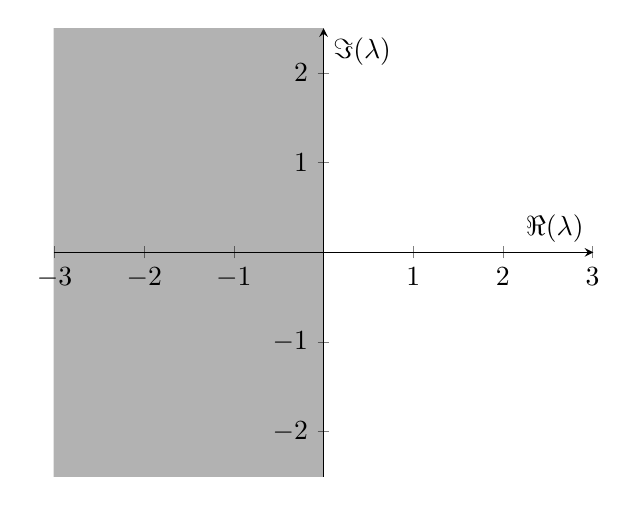
\begin{tikzpicture}
\begin{axis}[
    xmin=-2.0,
    xmax=2.0,
    ymin=-2.5,
    ymax=2.5,
    axis equal,
    axis lines=middle,
    xlabel=$\Re(\lambda)$,
    ylabel=$\Im(\lambda)$,
    disabledatascaling
]
\fill [opacity=0.3] (0.0,2.5) rectangle (-3.5,-2.5);
\end{axis}
\end{tikzpicture}
\caption{\label{fig:stability-linear-system-ct}Stability region of a linear system in continuous time.}
\end{figure}

In practice, measurements and controls are performed at discrete time points. In this case we are interested in the problem formulation in \emph{discrete time}. Representing a given solution step by index $i$, we have that $x(i+1)=\tilde{\mathbf{A}}x(i)$. It is simple to show that $\tilde{\mathbf{A}}=\exp(\mathbf{A}\tau)$, where $\tau$ is the sampling interval. Applying the time-stepping relationship recursively we find that at the $k-$th time step the solution can be expressed as $x(k)=\tilde{\mathbf{A}}^{k}x(0)$.

To investigate the stability in discrete time, we apply the same transformation as done in previous section but now applied to $\tilde{\mathbf{A}}$. This matrix can be rewritten as $\tilde{\mathbf{A}}=\tilde{\mathbf{T}}\tilde{\mathbf{D}}\tilde{\mathbf{T}}^{-1}$ from which one can show again that $\tilde{\mathbf{A}}^{k}$ depends only on $\tilde{\mathbf{D}}^{k}$. Writing the eigenvalues of $\tilde{\mathbf{D}}$ in exponential form $\lambda_{n}=R_{n}\exp(i\theta)$ leads to $\lambda_{n}^{k}=R_{n}^{k}\exp(ik\theta)$. In this expression, the exponential part is again related to oscillatory behavior only and the absolute value $R_{n}$ governs stability. Thus we conclude that in discrete time the unconditional stability arises when all $R_{n}<1$. This region is depicted in complex plane in Figure~\ref{fig:stability-linear-system-dt}.

\begin{figure}[h!]
\centering%
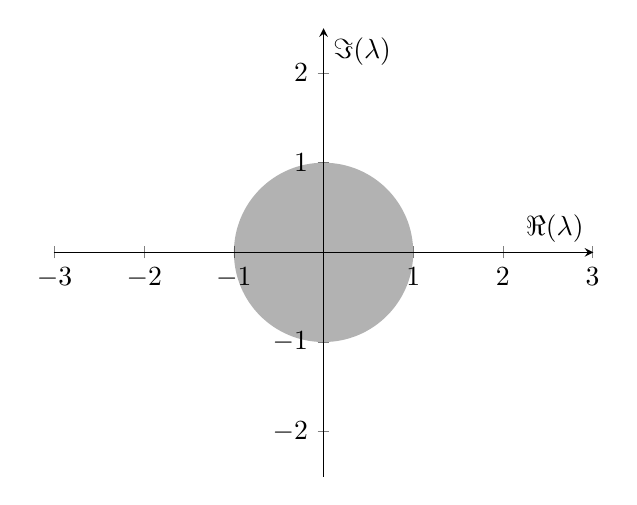
\begin{tikzpicture}
\begin{axis}[
    xmin=-2.0,
    xmax=2.0,
    ymin=-2.5,
    ymax=2.5,
    axis equal,
    axis lines=middle,
    xlabel=$\Re(\lambda)$,
    ylabel=$\Im(\lambda)$,
    disabledatascaling
]
\fill [opacity=0.3] (0,0) circle [radius=1];
\end{axis}
\end{tikzpicture}
\caption{\label{fig:stability-linear-system-dt}Stability region of a linear system in discrete time.}
\end{figure}

\endinput

\newSection{Thermodynamics}
\subsection{Fundamentals of Calphad}

\endinput
\subsection{Oxide systems for minerals}

\textcite{Huang1995} provide an assessment of \ch{CaO - MgO - SiO2} system at atmospheric pressure. The authors make use of a two-sublattice model for ionic liquid since it presents ions of different charges, and solid phases as ionic compounds with oxygen as anion and metals representing the cations. This can be achieved through an extension of \emph{compound energy model}.

\endinput

\newSection{Transport Phenomena}
\subsection{Dimensionless numbers}

\paragraph{Knudsen}: Particles mean free path over system characteristic dimension. Division between rarefied gas (Boltzmann) and continuum mechanics (Navier-Stokes).

\paragraph{Prandtl}: Ratio of momentum diffusivity to thermal diffusivity $\mathrm{Pr}=\sfrac{\nu}{\alpha}$. High $\mathrm{Pr}$ indicates that momentum transfer is more effective than heat transfer (oils), while low values (liquid metals) indicate thermal boundary layer is more important than viscous one.

\paragraph{\href{https://en.wikipedia.org/wiki/Nusselt_number}{Nusselt}}: Ratio of convective to conductive heat transfer at a boundary in a fluid, defined as $\mathrm{Nu}=\sfrac{hL}{k}$. Often in buoyancy-driven flow analysis it is correlated as $\mathrm{Nu}=a\mathrm{Ra}^b$. A Nusselt number of value one represents heat transfer by pure conduction. Increasing this number implies a laminar conductive-dominant flow and then a convective dominant turbulent flow.

\paragraph{\href{https://en.wikipedia.org/wiki/Grashof_number}{Grashof}}: Ratio of buoyancy to viscous forces defined as $\mathrm{Gr}=\sfrac{g\beta(T_s-T_{\infty})L^3}{\nu^2}$ and is analogous to Reynolds number in natural convection. Increasing the value of this number above a given threshold promotes buoyancy driven flow. 

\paragraph{\href{https://en.wikipedia.org/wiki/Rayleigh_number}{Rayleigh}}: Product of Grashof $\mathrm{Gr}$ and Prandtl $\mathrm{Pr}$ numbers. Related to the transition from laminar to turbulent in buoyancy-driven flows. Laminar to turbulent is assumed to take place at $10^9$~\cite{Balaji2014}.

\endinput
\subsection{About \textcite{Ergun1952}}

%TODO

\subsection{About \textcite{Gunn1978}} 

%TODO

\subsection{Multiphase modeling of dense granular media in gases}

This section discusses the physical modeling of dense granular media transport applied to multiphase CFD simulations. This is a particularly complex field because dynamic response of same material solid particles respond differently to flow field depending on their size, \emph{i.e.} they can be treated as separate phases. It is easy to understand this if you think of a dense bed where particles of different sizes will have coordination numbers that differ. In what follows, focus on gas-solid flows with high solid content will be given. This includes, but is not restricted to \begin{inparaenum}[(i)] \item pneumatic transport (dune/slug flow), \item fluidized/dense bed \end{inparaenum} flows. The case of particle-laden (particles in a continuous gas) is not treated here since particles are dispersed. There are two main approaches for modeling these sort of flows \begin{inparaenum}[(i)] \item Euler-Lagrange, and \item Euler-Euler\end{inparaenum}. In the first, fluid is treated as a continuum (thus Euler in the name) and particles are tracked individually (Lagrangian approach). From this explanation, one may correctly guess that Euler-Euler approach by its term describes both phases as interpenetrating continua, introducing the notion of phase fraction that is solved over computational domain. A detailed discussion of the subject is given by \textcite{Crowe2011}.

\subsubsection{Selecting an Euler-Euler model and solver in Ansys Fluent}

For the case of granular flows, the system of equations closure is achieved by application of kinetic theory adapted to macroscopic scale. Thus, several of the topics we discuss in this section are related to it and sometimes adapted from molecular dynamics. Ansys Fluent Euler-Euler models suitable for granular flow include the Mixture Model and Eulerian Model. Notice that these models cannot treat particle combustion, phenomenon that must use a DPM approach. Solidification and melting are also not supported.

Mixture Model is best suited for low loading flows, such as particle-laden and cyclone separators. It is also less computationally expensive than its counterpart and should be selected whenever in its applicability range. Eulerian Model is the most complex and general multiphase model in Fluent. Momentum is solved individually for each phase and coupling is achieved through pressure and interphase exchange coefficients. It can be used to model particle suspension and fluidized/dense beds. Since focus is given on dense granular media, Eulerian Model must be selected because particles are concentrated only in certain portions of the flow field. It is then selected as the \emph{right} choice for the case being treated here.

To justify this choice we first evaluate the particulate loading or mass concentration\footnote{As it is referred to in reference \cite{Crowe2011}.} $\beta$ given by the ratio of relative specific weights of dispersed phase $d$ and carrier $c$:

\begin{equation}
\beta=\frac{\rho_{d}\alpha_{d}}{\rho_{c}\alpha_{c}}
\end{equation}

\noindent{}where $\alpha$ denote the volume phase fraction and $\rho$ the specific weight. For a typical gas-solid flow in a dense bed $\beta>1000$ and high loading implies the use of Eulerian model. The inter-particle space~\cite{Crowe2011} can be estimated from dispersed phase volume fraction as

\begin{equation}
\frac{L}{d}=\left(\frac{\pi}{6\alpha_{d}}\right)^{\frac{1}{3}}
\end{equation}

For dense beds where $\alpha_{d}>0.5$ we have $\sfrac{L}{d}\le{}1$, meaning particles are in contact. Under such conditions two-way coupling of transport is required with addition of particle pressure and viscous stresses due to particles, what is only handled by the Eulerian Model.

Because of its complexity, higher order spatial and time discretization schemes are necessary. Second order time scheme is implemented using a Euler backward approximation in Fluent. Although a fully coupled solver is available, it is not as robust as the others for multiphase flows. In that case the best option is PC SIMPLE. In the case of steady-state solution, reducing the Courant number to as low as 4 can be useful for smooth convergence. If using PC SIMPLE, low under-relaxation of volume fraction is required, but that would dramatically increase computation time if using coupled solver.

\subsubsection{Setting up Eulerian Model for dense granular flows in Fluent}

Eulerian Model supports any number of secondary phases, thus if poly-dispersed particles are to be modeled they can be treated as separate phases, as discussed in the introduction. A single pressure is shared by all phases and momentum and continuity are solved for each phase. Setting up the interactions of solid phases between themselves and with the fluid requires additional models and related parameters. All $k-\varepsilon$ and $k-\omega$ are available and may apply to all phases or mixture.

Momentum conservation equation must include lift, wall lubrication, and turbulent dispersion forces. Virtual mass force can be neglected in this case because secondary phase is denser than carrier. Given the interactions between phases, an additional term is added to model those forces. This section will guide the selection of required models for the dense bed application. It must be emphasized that at the present there is no general formulation in the literature and these models are mostly empirically based.

For a single fluid dense bed reactor only fluid-solid exchange coefficients $K_{sl}$ are required, so we will not treat the fluid-fluid models in what follows. In its general form this coefficient is expressed as

\begin{equation}
K_{sl}=\frac{\rho_{s}\alpha_{s}}{\tau_{s}}f\quad\text{where}\quad\tau_{s}=\frac{\rho_{s}d_{s}^{2}}{18\mu_{l}}\implies{}K_{sl}=\frac{18\alpha_{s}\mu_{l}}{d_{s}^{2}}f
\end{equation}

\noindent{}where the first denominator $\tau_{s}$ represents the particulate relaxation time. From this equation we see that viscous fluids and high particulate contents increase the interaction, while larger particles reduce it. The factor $f$ is a function of drag coefficient $C_{D}$ and it is the law describing it that must be adapted for the present case. Most common option is \textcite{Syamlal1989} model which should only be used in conjunction of solid shear stresses kinetic component as defined by \textcite{Syamlal1993}, also the default. Although the model by \textcite{Wen1966} is not applicable to dense systems, an improvement proposed by \textcite{Gidaspow1992} through the use of \textcite{Ergun1952} equation allows the application to densely packed systems, better suited for the present case.
%TODO check Fluent EMMS appliability too.

Regarding solid-solid exchanges, coefficient $K_{ls}$ is computed taking into account the pair-wise restitution coefficient, the friction coefficient, and particle sizes~\cite{Syamlal1987b}. Drag modification does not seem required in the present context. Lift correction, wall lubrication model, and virtual mass are all non-applicable because they concern only liquid-gas systems, specially droplets and bubbles. Lift force modeling is also discarded because in dense bed reactors particle distances are small, same reason for why we may neglect turbulent dispersion corrections. Since in dense beds the kinetics theory application to particles is less relevant, then a granular temperature set to a constant low value. Impacts of this on shear stress are discussed in what follows.

% NOTE: in Fluent Theory Guide it is not Lun, but Gidaspow, although the option does not exist in the corresponding version of the software. For now I did not yet check the actual papers to understand if that factor really exists.
In cases where solids volume fraction is below the packing limit, the granular flow is said to be in compressible regime. In that case a solids pressure is computed independently and added by Ansys Fluent in the momentum equation. The most important parameter intervening in this case is the coefficient of restitution $e_{ss}$. Formulations are presented by \textcite{Lun1984}, \textcite{Syamlal1993}, and \textcite{Ahmadi1990}. For one solid phase the radial distribution function $g_{0}$ proposed by \textcite{Lun1984} is to be used.

Solids shear stress contains terms due to translation and collision. Pure collision term is modeled as proposed by \textcite{Gidaspow1992}. For its kinetic component the default model is the one by \textcite{Syamlal1993} and the one by \textcite{Gidaspow1992} is also available. The component of bulk viscosity  is by default zero and can be included through the model by \textcite{Lun1984}. Once a threshold frictional packing limit is reached, a corresponding term is added, by default as per \textcite{Schaeffer1987} to account for the viscous-plastic transition that occurs. It is recommended to apply this term because at solid fraction the application of kinetic theory is no longer relevant and frictional stresses need to be considered. The associated frictional pressure is mainly semi-empirical and models are provided by \textcite{Johnson1987} and \textcite{Syamlal1993}. If using one of the models by \textcite{Lun1984} or \textcite{Gidaspow1992} for the radial distribution function, the Ansys Fluent provides an \emph{based-ktgf} model for handling high packing fraction solids pressure.
 
Heat transfer in granular flow can be described through the Nusselt number correlation proposed by \textcite{Gunn1978}. Notice that this is applicable to Reynolds numbers below $10^5$. Thermal conductivity $\kappa_q$ of phases is then required as a parameter.

To close the set of required closure models one needs to select a turbulence description. Since we are discussing granular multiphase flow, turbulence applies only to the primary gas phase. Standard $k-\varepsilon$ or $k-\omega$ models can be selected and no turbulence interaction parameters are required.

In summary, the multiphase parameters from Table~\ref{tab:eulerian-dense-bed} can be selected in Ansys Fluent for the granular phases (each particle diameter for the same physical phase of matter being considered a separate granular phase).

\begin{table}[!ht]
\caption{\label{tab:eulerian-dense-bed}Models for Eulerian granular dense bed.}
\small\centering%
\begin{tabular}{lcc}
\toprule[2pt]
  \textbf{Parameter}
& \textbf{Model}
& \textbf{References}
\\
\midrule[1pt]
\multicolumn{3}{c}{\textbf{Granular (solid) phase description}}\\
\midrule
  Granular Temperature Model
& \Verb|Phase Property|
&
\\[6pt]
  %OK
  Granular Viscosity
& \Verb|gidaspow|
& \cite{Gidaspow1992}
\\[6pt]
  %OK
  Granular Bulk Viscosity
& \Verb|lun-et-al|
& \cite{Lun1984}
\\[6pt]
  %OK
  Solids Pressure
& \Verb|lun-et-al|
& \cite{Lun1984}
\\[6pt]
  %OK
  Granular Temperature
& \Verb|algebraic|
&
\\[6pt]
  %OK
  Frictional Viscosity
& \Verb|schaeffer|
& \cite{Schaeffer1987}
\\[6pt]
  %OK
  Frictional Pressure
& \Verb|based-ktgf|
& 
\\[6pt]
  %OK
  Friction Packing Limit
& \Verb|0.61|
&
\\[6pt]
  %OK
  Angle Of Internal Friction
& \Verb|30.0|
&
\\[6pt]
  %OK
  Packing Limit
& \Verb|0.63|
&
\\[6pt]
  %OK
  Radial Distribution
& \Verb|lun-et-al|
& \cite{Lun1984}
\\[6pt]
  %OK
  Frictional Modulus
& \Verb|derived|
&
\\[6pt]
  %OK
  Elastic Modulus
& \Verb|derived|
&
\\
\midrule
\multicolumn{3}{c}{\textbf{Phase interactions -- Forces between fluid-solid}}\\
\midrule
  Drag Coefficient
& \Verb|gidaspow|
& \cite{Ergun1952,Wen1966,Gidaspow1992}
\\[6pt]
  Drag Coefficient Modification
& \Verb|none|
& 
\\[6pt]
  Lift Coefficient
& \Verb|none|
& 
\\[6pt]
  Wall Lubrication
& \Verb|none|
& 
\\[6pt]
  Turbulence Interaction
& \Verb|none|
& 
\\[6pt]
  Virtual Mass Coefficient
& \Verb|none|
& 
\\[6pt]
  Surface Tension Coefficient
& \Verb|none|
& 
\\
\midrule
\multicolumn{3}{c}{\textbf{Phase interactions -- Forces between solid-solid}}\\
\midrule
  Restitution Coefficient
& $<0.5$ for hot brittle phases
& 
\\
\midrule
\multicolumn{3}{c}{\textbf{Phase interactions -- Heat transfer between fluid-solid}}\\
\midrule
  Heat Transfer Coefficient
& \Verb|gunn|
& \cite{Gunn1978}
\\
\midrule
\multicolumn{3}{c}{\textbf{Phase interactions -- Interfacial area between fluid-solid}}\\
\midrule
  Interfacial Area
& \Verb|ia-particle|
& 
\\
\bottomrule[2pt]
\end{tabular}
\end{table}

\endinput
\subsection{Meshing in Ansys Fluent}

\subsubsection{Dynamical meshing for a linear movement}

Ansys Fluent supporting documentation for moving bodies is mainly focused on rotating parts (turbo-machinery) and falling bodies (aerodynamics). Instructions for parts moving linearly is quite limited, as online tutorials. \href{https://www.youtube.com/watch?v=fbaV_knzzks}{This video} provides a good basis for modeling this sort of movement. In this section we discuss some ideas and provide a basic checklist with aspects to consider when modeling a system containing a plug-like moving part.

\begin{itemize}
\item It is a good idea to split domain into multiple parts to avoid remeshing zones far from the moving parts or where the movement is irrelevant. This can provide an important computational effort reduction.

\item When setting up the case, do not forget to set up the deformation movement of the zone where parts are moving so that the smoothing of mesh is propagated in the region.

\item Use of layering with a good peel layer thickness estimation is almost a requirement for successful simulation of a plug-like system.

\item Do not forget that the macro \verb+DEFINE_CG_MOTION+ can only be used when compiled (it is incompatible with interpreted macro loading).

\item Structured boundary layers can be set as stationary zones if re-meshing is undesirable.

\item In most cases you should set remeshing interval to unity or activate implicit update (and accept the high computational overhead associated to it).

\item To avoid movement of a part that crosses or touches a wall, it might be useful to consider a zone where fluid should not flow through as a porous zone (parametrized in an UDF) with closed porosity.
\end{itemize}

\endinput

\newSection{Molecular Dynamics}

\newpage%
\printbibliography%
\end{document}